\documentclass[journal]{IEEEtai}

\usepackage[colorlinks,urlcolor=blue,linkcolor=blue,citecolor=blue]{hyperref}
\usepackage{float}
\usepackage{color,array}
\usepackage{cite}
\newcommand{\tabitem}{~~\llap{\textbullet}~~}
\usepackage{graphicx}
\usepackage{tikz}
\usepackage{caption}
\usepackage{comment}

\usepackage{booktabs, makecell, multirow, tabularx}
\newcolumntype{C}{>{\centering\arraybackslash}X} % centered version of "X" type
\newcommand\mcx[1]{\multicolumn{1}{C}{#1}}
\setlength{\extrarowheight}{1pt}
\usepackage{stfloats}
\usepackage{siunitx}
\usepackage{caption}
\newcommand{\ap}[1]{AP\textsubscript{#1}}
\newcommand{\apavg}[0]{AP\textsubscript{\(\!\varnothing\)}}


%% \jvol{XX}
%% \jnum{XX}
%% \paper{1234567}
%% \pubyear{2020}
%% \publisheddate{xxxx 00, 0000}
%% \currentdate{xxxx 00, 0000}
%% \doiinfo{TQE.2020.Doi Number}

\newtheorem{theorem}{Theorem}
\newtheorem{lemma}{Lemma}
\setcounter{page}{1}
%% \setcounter{secnumdepth}{0}



\usepackage[backend=bibtex, style=ieee]{biblatex}
\addbibresource{library}

\begin{document}


\title{Bankruptcy prediction in Colombian case, using multilayer perceptron trained with memetic algorithm} 


\author{ Iván andrés Trujillo \IEEEmembership{PUJ MINTA}}

\author{Student:Iván Andrés Trujillo Abella,\\

\\
\\

Proffesors: Eliana María González Neira \& Gabriel Mauricio Zambrano Rey}
\maketitle

\begin{abstract}
Literature about Bankruptcy prediction is still incipient, therefore this work try to fill this gap by using machine learning  and metaheuristics techniques to find an optimal set of  weights in a MLP model.
\end{abstract}


\begin{IEEEkeywords}
Machine learning, Bankruptcy, Metaheuristics, Evolutionary Algorithms, Local Search, Memetic algorithms, Neural Networks, Multilayer Perceptron.
\end{IEEEkeywords}





\section{Information(Data)}

Data was retrieved from SIS by the period 2016-2019, classifying as bankrupt all Small and Medium Enterprises(SMEs) firms  that were declared some process different to active or preoperative state.


To predict bankruptcy, financial ratios from one and two years before the occurrence of the event were used(in different models). For instance, for those firms that entered into a process in 2019,  the financial ratios of 2018 and 2017 were used to train the models.


For those firms that did not experience the event (controls), the mean of the financial ratios was used based on their period of activity. For instance, if firm $j$ entered into database in 2017 and did not experience the event, the mean of the financial ratios for the period (2017 - 2019) was used.
\subsection{Exclusion criteria}

\begin{itemize}

\item Financial information reported on a date different from December 31 of each year was excluded.

\item Firms declared to be in a preoperative condition each year were excluded from the database.

\item  Firms that presented the event for the initial year(2016) were excluded from the database.

\item Firms that present missing values and not valid financial ratios were excluded from database.
\end{itemize}


\section{Description of data}

To describe categorical data, absolute and relative frequencies were used. The numerical variables were described using the mean and standard deviation if the variable is normally distributed; otherwise, the median, 25th percentile, and 75th percentile were used.

To compare the financial ratios among non-bankrupt and bankrupt firms and determine if there are significant differences among them, we used t-tests or the Wilcoxon rank sum test if the variable is normal or not, respectively.
To test the normality of variables, we used the Shapiro-Wilk test. To determine if there is independence between the event and categorical variables, the $\chi^{2}$ test was used.

Finally, to test if there is correlation(monotonicity) among numerical variables the spearman coefficient was used.


\subsection{Variables  (Financial ratios)}
Financial ratios could be categorized in some groups, for instance \textit{liquidity, leverage} and \textit{profitability } for this work were used:




\subsubsection{liquidity ratios}
Measure the firm ability to pay its financial obligations;
Current ratio and Ratio of short-term liabilities were used.
\end{itemize}

\subsubsection{Profitability ratios}
Measure the firm ability to generate incomes;
Gross profit margin, Net profit margin, Return on equity and Return on asset were used.



\subsubsection{Leverage ratios}
Measure the level of debt in long run;
Debt equity ratio and Indebtedness ratio were used.

Were also added two classic financial ratios in bankruptcy prediction used by Altman; named in this work Altman $x_{1}$ and Altman $x_{2}$.

The following Table (\ref{ratios}) described each one of the aforementioned ratios, according to NIFF financial statements retrieved for this work.

\begin{table*}[!h]
\caption{Financial ratios definition}
\label{ratios}
\setlength\tabcolsep{5pt}
\def\arraystretch{2} 
\ContinuedFloat
\centering
\begin{tabularx}{\linewidth}{CC}
\toprule
Ratio      & Definition    \\
\cmidrule{1-2}

Gross Profit Margin (GPM)             &
$\frac{\text{Gross profit}}{\text{Operating revenues}}$                                \\
Net Profit Margin (NPM)              
& $\frac{\text{Profit(Loss)}}{\text{Operating revenues}}$                                \\
Return On Equity (ROE)               
& $\frac{\text{Profit(Loss)}}{\text{Total equity}}$                                      \\
Return On Assets (ROA)               
& $\frac{\text{Profit(Loss)}}{\text{Total assets}}$                                      \\
Indebtedness Ratio (IR)              
& $\frac{\text{Total liabiliaties}}{\text{Total assets}}$                                \\
Debt Equity Ratio (DER)              
& $\frac{\text{Total liabiliaties}}{\text{Total equity}}$                                \\
Current Ratio (CR) & 
$\frac{\text{Total current assets}}{\text{Total current liabilities}}$                               
\\
Ratio of Short-Term Liabilities (RSL) & 
$\frac{\text{Total current liabilities}}{\text{Total liabilities}}$                                \\

Altman $x_{1}$$                                   & 
$\frac{\text{Total current assets - Total current liabilities}}{\text{Total assets}}$ \\
Altman $x_{2}$                            
& $\frac{\text{Accumulated  profits}}{\text{Total liabilities}}$                 \\
\bottomrule
\end{tabularx}
\end{table*}


\section{Modeling prediction}
The models used to compare prediction performance on bankruptcy were: Decision tree, logistic regression and multilayer perceptron.

 was constructed a grid search.

\subsection{Train and test}

We used 70\% to train and 30\% to test.


\subsection{Hyperparameter tunning}

\subsection{Logistic regresion}


\subsection{Multilayer perceptron}


\subsection{Decision tree}
-
	

\subsection{Balance data}

To handle the unbalanced data used \text{undersampling}


\section{Results}

From  a total sample of 27,210 firms, of which 1,279 were classified as bankrupt, only 16,488 of which 318 were bankrupt represented the final sample. 


The following Figure (\ref{flowchart}) describe the process to obtain the final data to modelling.


\usetikzlibrary{shapes.geometric, arrows}

\tikzstyle{startstop} = [rectangle, rounded corners, 
minimum width=3cm, 
minimum height=1cm,
text centered, 
draw=black, 
fill=red!30]

\tikzstyle{io} = [ rectangle, minimum width=3cm, 
minimum height=1cm, text centered, 
draw=black, fill=white!30]

\tikzstyle{process} = [rectangle, 
minimum width=3cm, 
minimum height=1cm, 
text centered, 
text width=3cm, 
draw=black, 
fill=white!30]

\tikzstyle{decision} = [rectangle, 
minimum width=3cm, 
text width = 3cm,
minimum height=1cm, 
text centered, 
draw=black, 
fill=gray!30]

\tikzstyle{arrow} = [thick,->,>=stealth]

\begin{figure}[h]
\caption{Flowchart processing data}
\label{flowchart}

\begin{tikzpicture}[node distance=2cm]
\node (box1) [process] {Initial database  
N = 27,210 
Bankrupt = 1279};
-\node (text1) [decision, left of=box1, xshift = -3cm] {Unique firms by period};
++
\node (box2) [process, below of=box1] {N = 26,702 
Bankrupt = 771
};

\node (text2) [decision, left of=box2, xshift = -3cm] {Without firms that bankrupt in 2016};




\node (box3) [process, below of=box2] {N = 17,613 
Bankrupt = 328};


\node (text3) [decision, left of=box3, xshift = -3cm] {Firms that have complete variables to modelling};


\node (box4) [process, below of=box3] {N = 16,488 
Bankrupt = 318};


\node (text4) [decision, left of=box4, xshift = -3cm] {Firms with valid financial ratios};

		
\draw [arrow] (text1) -- (box1);
\draw [arrow] (box1) -- (box2);
\draw [arrow] (text2) -- (box2);
\draw [arrow] (box2) -- (box3);
\draw [arrow] (text3) -- (box3);
\draw [arrow] (box3) -- (box4);
\draw [arrow] (text4) -- (box4);
\end{tikzpicture}
\end{figure}






The Figure (\ref{corrmatrix})  show the  spearman coefficient among numerical financial ratios.


\begin{figure}[h]
\caption{Spearman correlation in predictor variables}
\label{corrmatrix}
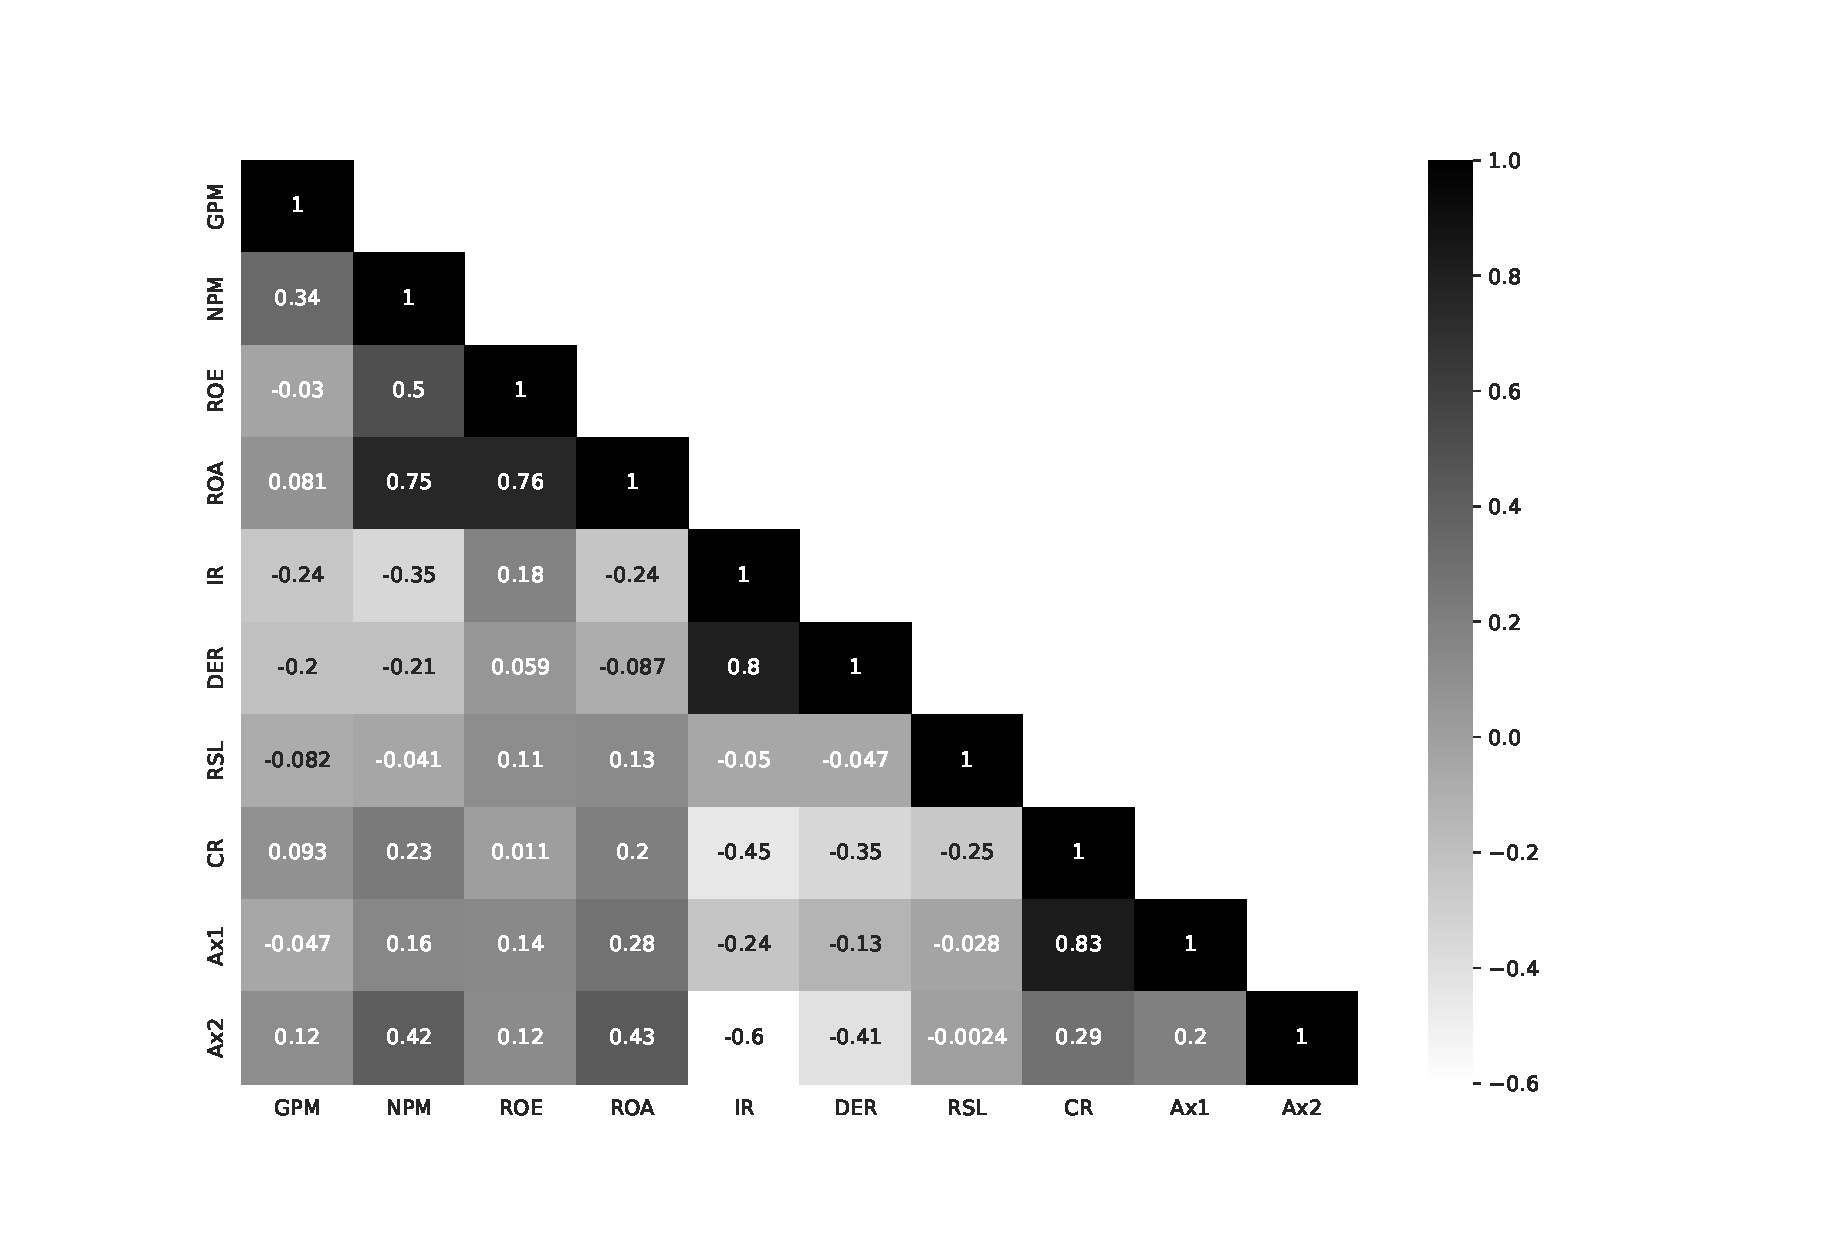
\includegraphics[scale=0.38]{Matrix.eps}
\end{figure}


The following Table \ref{tableone} show the difference among the financial ratios of one year before of the bankrupt and the mean of the ratios by the period of activity in no-bankrupt firms.
The results indicate that there are significative difference in all ratios, and no independence among the event and the sector.


% word with c and l
\begin{table*}[h]
    \caption{Year of bankrupt, financial ratios and sector among groups}
    \label{tableone}
\setlength\tabcolsep{15pt}
\ContinuedFloat
    \centering
\begin{tabular*}{\textwidth}{@{}*{7}{c}} 
\toprule
& & & & \multicolumn{2}{c}{Grouped by event} \\
 \cmidrule{5-6}
 &  & Missing & Overall & No-bankrupt & Bankrupt & P-Value \\
n &  &  & 16806 & 16488 & 318 &  \\
\cline{1-7}

\multirow[t]{4}{*}{time-event, n (\%)}  & 0.0 & 0 & 16488 (98.11) & 16488 (100.00) &  & <0.001 \\
 & 2017.0 &  & 99 (0.59) &  & 99 (31.13) &  \\
 & 2018.0 &  & 96 (0.57) &  & 96 (30.19) &  \\
 & 2019.0 &  & 123 (0.73) &  & 123 (38.68) &  \\
 
GPM, median [Q1,Q3] &  & 0 & 0.31 [0.18,0.56] & 0.32 [0.18,0.56] & 0.26 [0.14,0.41] & <0.001 \\
NPM, median [Q1,Q3] &  & 0 & 0.03 [0.00,0.08] & 0.03 [0.00,0.08] & -0.02 [-0.18,0.03] & <0.001 \\
ROE, median [Q1,Q3] &  & 0 & 0.07 [0.01,0.16] & 0.07 [0.01,0.16] & 0.01 [-0.18,0.09] & <0.001 \\
ROA, median [Q1,Q3] &  & 0 & 0.03 [0.00,0.06] & 0.03 [0.00,0.07] & -0.01 [-0.09,0.01] & <0.001 \\
IR, median [Q1,Q3] &  & 0 & 0.53 [0.32,0.72] & 0.52 [0.32,0.72] & 0.74 [0.59,0.88] & <0.001 \\
RSL, median [Q1,Q3] &  & 0 & 0.75 [0.45,0.98] & 0.75 [0.45,0.98] & 0.53 [0.28,0.87] & <0.001 \\
Ax1, median [Q1,Q3] &  & 0 & 0.22 [0.04,0.43] & 0.22 [0.04,0.43] & 0.09 [-0.08,0.28] & <0.001 \\
Ax2, median [Q1,Q3] &  & 0 & 0.19 [0.04,0.40] & 0.19 [0.05,0.40] & 0.04 [-0.12,0.18] & $<$0.001 \\


\multirow[t]{20}{*}{Sector, n (\%)} & A & 0 & 1012 (6.02) & 990 (6.00) & 22 (6.92) & <0.001 \\
 & B &  & 282 (1.68) & 277 (1.68) & 5 (1.57) &  \\
 & C &  & 2735 (16.27) & 2647 (16.05) & 88 (27.67) &  \\
 & D &  & 10 (0.06) & 10 (0.06) &  &  \\
 & E &  & 28 (0.17) & 27 (0.16) & 1 (0.31) &  \\
 & F &  & 2238 (13.32) & 2190 (13.28) & 48 (15.09) &  \\
 & G &  & 5288 (31.46) & 5201 (31.54) & 87 (27.36) &  \\
 & H &  & 314 (1.87) & 310 (1.88) & 4 (1.26) &  \\
 & I &  & 363 (2.16) & 349 (2.12) & 14 (4.40) &  \\
 & J &  & 464 (2.76) & 456 (2.77) & 8 (2.52) &  \\
 & K &  & 474 (2.82) & 473 (2.87) & 1 (0.31) &  \\
 & L &  & 1449 (8.62) & 1443 (8.75) & 6 (1.89) &  \\
 & M &  & 1142 (6.80) & 1127 (6.84) & 15 (4.72) &  \\
 & N &  & 646 (3.84) & 632 (3.83) & 14 (4.40) &  \\
 & O &  & 4 (0.02) & 4 (0.02) &  &  \\
 & P &  & 87 (0.52) & 86 (0.52) & 1 (0.31) &  \\
 & Q &  & 64 (0.38) & 63 (0.38) & 1 (0.31) &  \\
 & R &  & 88 (0.52) & 86 (0.52) & 2 (0.63) &  \\
 & S &  & 115 (0.68) & 114 (0.69) & 1 (0.31) &  \\
 & U &  & 3 (0.02) & 3 (0.02) &  &  \\
\bottomrule
\end{tabular*}
\end{table*}



The following table (\ref{imbalanced}) show us the performance of the models with the variables used to predict bankruptcy, the result indicate a lower performance to predict correctly the bankrupt firms.



\begin{table*}[h]	
	\caption{Models performance over imbalanced data}
    \label{imbalanced}
\ContinuedFloat
    \centering
\begin{tabularx}{\linewidth}{lCCCCCCl}
\toprule
 \multicolumn{1}{c}{}& \multicolumn{2}{c}{Logistic Regression} & \multicolumn{2}{c}{Decision Tree} & \multicolumn{2}{c}{Multilayer Perceptron}\\
\cmidrule(lr){2-3}   \cmidrule(lr){4-5}  \cmidrule(lr){6-7} \\
 &No-Default & Default & No-Default & Default & No-default & Default \\
\midrule
precision & 0.98 & 0.15 & 0.98 & 0.06 & 0.98 & 0.00 \\
recall & 1.00 & 0.03 & 0.94 & 0.18 & 1.00 & 0.00 \\
f1-score & 0.99 & 0.05 & 0.96 & 0.09 & 0.99 & 0.00 \\
support & 4947.00 & 95.00 & 4947.00 & 95.00 & 4947.00 & 95.00 \\ 
\bottomrule
\end{tabularx}
\end{table*}


The following Table (\ref{balanced}) shows that all models have major performance.


\begin{table*}[h]	
	\caption{Models performance over balanced data using undersampling}
    \label{balanced}
\ContinuedFloat
    \centering
\begin{tabularx}{\linewidth}{lCCCCCCl}
\toprule
 \multicolumn{1}{c}{}& \multicolumn{2}{c}{Logistic Regression} & \multicolumn{2}{c}{Decision Tree} & \multicolumn{2}{c}{Multilayer Perceptron}\\
\cmidrule(lr){2-3}   \cmidrule(lr){4-5}  \cmidrule(lr){6-7} \\
 &No-Default & Default & No-Default & Default & No-default & Default \\
\midrule
precision & 0.68 & 0.72 & 0.71 & 0.64 & 0.72 & 0.76 \\
recall & 0.75 & 0.64 & 0.58 & 0.76 & 0.78 & 0.69 \\
f1-score & 0.71 & 0.68 & 0.64 & 0.70 & 0.75 & 0.73 \\
support & 96.00 & 95.00 & 96.00 & 95.00 & 96.00 & 95.00 \\  
\bottomrule
\end{tabularx}
\end{table*}





\newpage
\printbibliography



\end{document}